% \chapter{History of the LHC}\label{sec:appendixLhc}
\newappendix{History of the LHC}\label{sec:appendixLhc}

The history of physics runs of LHC is the description of the laboratory conditions under which ATLAS collected data.
It is also an interesting narrative of a tightly coupled process of developing and testing collider engineering principles.
The dramatic improvement of the machine's performance over the years of its operation is a testament to the efficacy of this strategy.

This section will first describe the LHC's first round of operation, Run 1.
Crucial machine developments were also made in Run 1 that lead to energy and luminosity increases improvements.
This section proceeds to describe the second round of operation, Run 2.
During Run 2, the machine provided collisions at unprecedented energy and intensity that haven enabled searches for new phenomena as well as precision measurements.

\section{Run 1}

The first run of the LHC took place between 2010 and 2013.
Collisions took place with beam energies between 3.5 and 4~TeV.\cite{lhcRun1}
Run 1 provided the collision data in which the Higgs boson was discovered. \cite{atlashiggs}
It also provided the basis for the steady improvement of the LHC.
For example, as a result of the experience gained from operating the machine, it was possible to gradually decrease the bunch spacing from 150~ns (2010), to 75~ns (2011) finally to 50~ns (2011/2012). \cite{lhcRun1}

The run began in 2010 with counter-rotating beams of energy 1.2~TeV.
This energy, which is below the design energy of 7~TeV per beam, was selected due to earlier damage during operation in 2008.
After verifying the stability of the machine, the energy was gradually increased to 3.5~TeV per beam.
The first physics ready collisions began on February 27, with just two bunches per beam and containing relatively few protons each.
Over several months, the number of bunches and the number of particles per bunch were increased.
The operation was not without difficulty: throughout the run, unidentified falling objects (UFOs) within the beam-pipe disrupted the beam and resulted in 60 beam dumps.
The UFO events are speculated to be caused by water vapor solidifying on the top of the beam-pipe and later fall through the beam.
Furthermore, unexplained and mysterious oscillations in the beam tune (called the ``hump'') plagued operators. \cite{lhcRun1}
The year ended with significant gains in the beam energy, bunch spacing, and bunch density.

The second year of the run began on February 19, 2011, with three weeks of recommissioning.
The first physics beams began on March 13 at 3.5 TeV and 32 bunches per beam.
This was gradually increased to 200 bunches, with 75~ns spacing.
The bunch density was also increased to 1.34$\times10^{11}$ ppb.
On April 21, the LHC reached an instantaneous luminosity of $4.6\times10^{33}~\cms$, which broke the previous record from the Tevatron.
It is at some time during 2011 that the hump disappeared from the tune plots, leaving the mystery unresolved.
Overall, the second year was the first to provide productive physics data. The mean stable beam time was 6.1 hours, which corresponds to 33\% efficiency.
In total, 5.6~\fb of data was provided. \cite{lhcRun1}

In the years 2012 and 2013, the investment in carefully developing the LHC paid off with a wealth of physics data.
The beam energy was increased to 4~TeV in order to increase the Higgs production cross-section.
The first stable beams at 4~TeV, holding only three bunches, were circulated on April 5, 2012.
After a month of commissioning, the first physics beams were provided on May 4.
The nominal beam design was 1374 bunches with 50~ns bunch spacing\footnote{Due to the arrangement of the bunches, only 1368 bunches collided inside ATLAS. At the time, there was also a plan to have private bunches colliding only in LHCb.}.
The bunch intensity was also increased to 1.7$\times10^{11}$ ppb, and the run stable beam efficiency was improved to 36.5\%.
% Emittance 2-2.5 microns

\begin{figure}[h!]
\captionsetup[subfigure]{position=b}
\centering
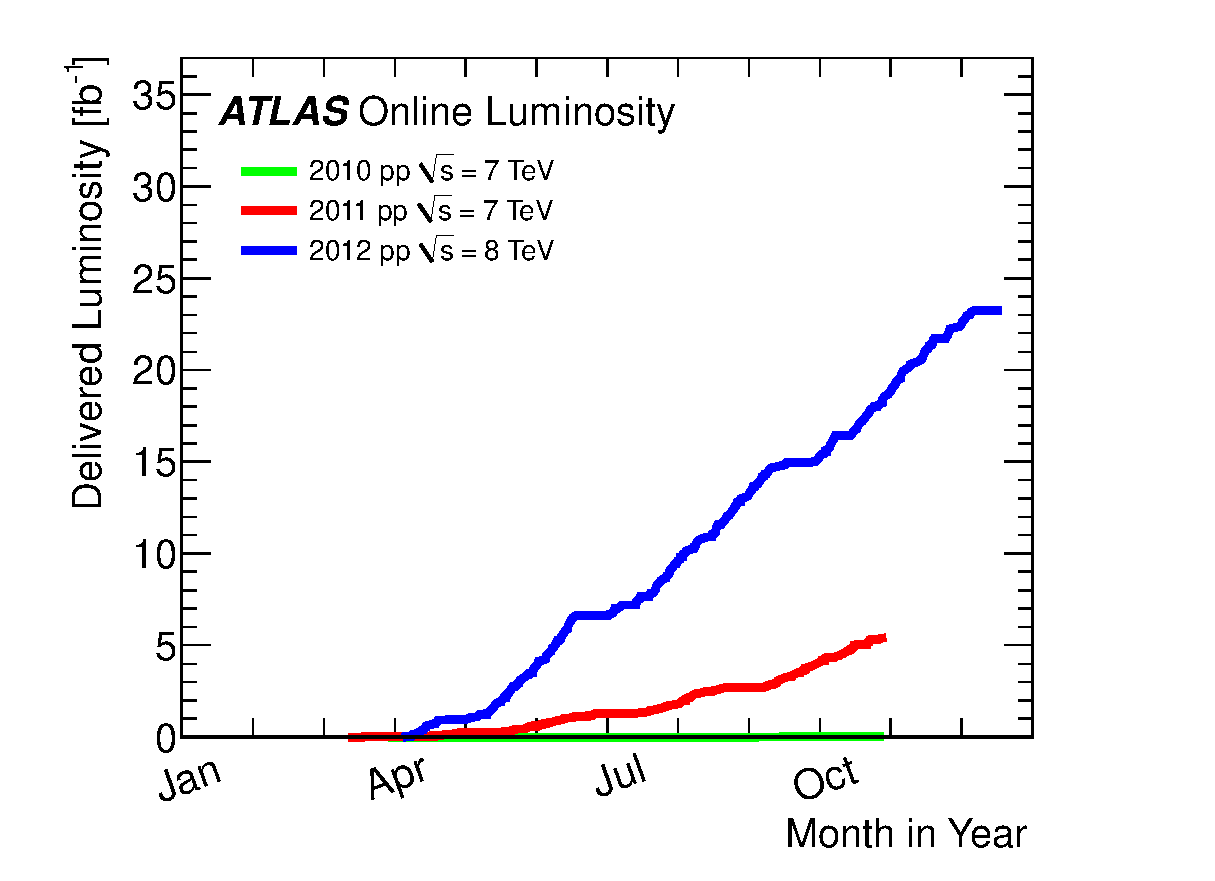
\includegraphics[width=0.8\textwidth]{figures/experiment/lhc/run1Lumi.eps}
\caption{The recorded luminosity by ATLAS during Run~1. The dramatic year-to-year improvement is clear from the slopes of the curves, indicating the rate at which data was recorded.}
\label{fig:run1Lumi}
\end{figure}

The performance of the LHC during Run 1 enjoyed dramatic improvement over time.
This is evident in Figure \ref{fig:run1Lumi}, which shows the integrated luminosity for various years, as recorded by ATLAS.
The rate at which the machine delivered data grew steadily due to the iterative study and tuning that took place during Run 1.
However, the machine operation was far from perfect, and the cryogenic system was most problematic, causing 25-30\% of all downtime, followed by the injector systems.
Resolving these issues was a major goal for Run 2. \cite{lhcRun1}

    % \item \textbf{Beam Cycle} (probably, should use run2 resource) \cite{lhcRun1}
    % \begin{itemize}
    %     \item Injection. Beam is ``scraped'' by transfer line collimator's. In run 1, about 2-4\% of the beam is lost. This done in SPS. The collimator jaws heat and outgas, so these are opened as soon as injection is finished. Rings are filled consecutively (as opposed to alternating bunches) because ALICE requested it (it reduces their background??). \cite{lhcRun1}
    %     \item Ramp. The ramping speed is limited by dipole current ramp rate of 10 A/s, which corresponds to 6 GeV/s. A ``flat top'' of 300 s, during which the tune decay is corrected for. \cite{lhcRun1}
    %     \item Separation/crossing angles. {\color{red} Warning, confused} Crossing angle is 170 micro radians. Separation is on the order of mm. Horizontal separation in P1,P2. Vertical in P5,P8. Hence in IR1 beam 1 moves downward/inside. \cite{lhcRun1}
    %     \item Collisions. When start, tails of bunches are expelled, leading to a brief drop in expected beam lifetime. The expected lifetime of the beam is optimized by reducing the chromaticity {\color{blue} \url{https://cds.cern.ch/record/302491/files/p77.pdf}(the change in linear parameters of transverse motion with beam energy).} HOW do they reduce chromaticity? \cite{lhcRun1}
    %     \item Tune. The beam is large during the ramp, and reduced during squeeze. \cite{lhcRun1}
    %     \item Collimators. Used for squeeze, used for betatron cleaning. Used to clean ``physics debris''. \cite{lhcRun1}
    % \end{itemize}
% \end{itemize}

\section{Run 2}

The second operation of the LHC took place between 2015 and 2018.
This run is characterized by higher beam energy: 6.5~TeV per beam throughout the run.
This is a monstrous amount of energy to concentrate into the protons that make up the beam.
To perform this feat with AA batteries, a proton would have to be transported down a stack that reached from Earth to the sun and then on to Mercury.
It is also characterized by innovative strategies to increase the delivered luminosity.
Key among these improvements are a small emittance and $\beta^*$ and reduced 20~ns bunch spacing.

The machine cycle begins with threading: the beam is injected with low bunch intensity and stopped on collimators at stages throughout the rings.
The trajectory is adjusted at each stop before proceeding to the next one.
Threading takes place primarily at the beginning of the year since fewer corrections are needed when the machine is in a steady state.
When a complete orbit can be made by a 12-bunch beam, the position of several orbits is averaged, and then adjusted, in a process called steering.
When the orbits are stable, the rest of the beam is injected \footnote{This is done sequentially, rather than simultaneously, for each beam. This is because simultaneous injection heated the injection collimators, causing them to off-gas.}.
When the complete beam has been injected, it undergoes a combined \emph{ramp and squeeze}\footnote{Combining ramp and squeeze was an innovation to increase the beam-on efficiency. Previously the squeeze was performed after ramping.}.
During ramp, the beam is accelerated while the dipole magnets simultaneously ramp up their fields.
The standard ramp time is 1210s. 
The ramping pattern is parabolic-exponential-linear-parabolic and takes approximately 20 minutes. 
During the squeeze, the beam optics are adjusted in steps to reach a particular $\beta^*\approx30$~cm target in the interaction regions.
The squeeze continues after the ramp.
Once it is complete, the beams are steered to collide.

During the whole process, the beam tune and chromaticity are delicately adjusted.
For example, the chromaticity is controlled to $\pm$2 during filling and has typical values of +20 during filling and +15 during operation. \cite{lhcRun2}
The positive chromaticity enhances beam stability, in particular head-tail instability within bunches.
% The SPS bunch spacing is 200-250~ns.

It is desirable to maintain a target luminosity (1.5\times{34}\cms), with a process called luminosity leveling.
This is accomplished by adjusting the crossing angle $\theta_c$ (introduced in 2017), and the value of $\beta^*$ (introduced in 2018).
Since the beam is extremely sensitive to perturbation, these adjustments are made in small steps of 10 micro radians, and $\approx3$~cm.
The beam is so sensitive to external sources that tidal effects, earthquakes, and HL-LHC civil engineering have all been observed in the radial orbit evolution over time, as shown in Figure \ref{fig:tides}.

\begin{figure}[h!]
\captionsetup[subfigure]{position=b}
\centering
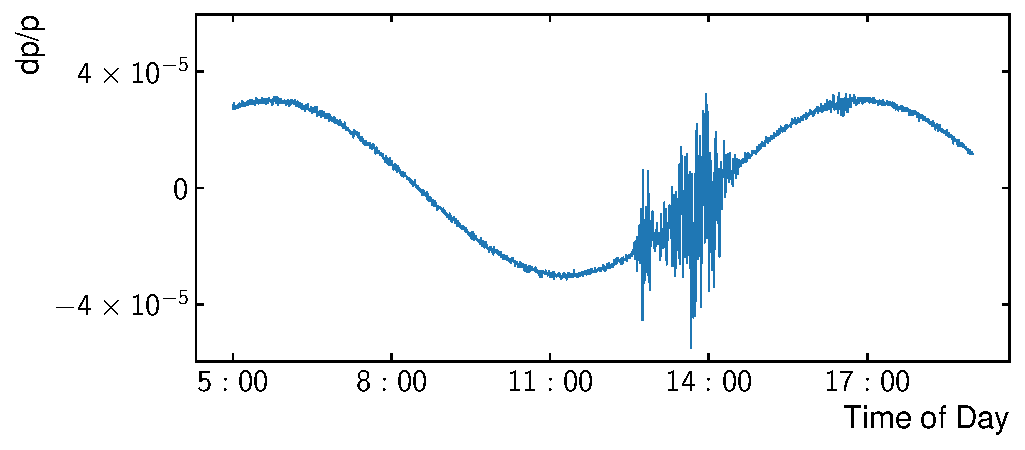
\includegraphics[width=0.95\textwidth]{figures/experiment/lhc/tides2.pdf}
\caption{Illustration of the evolution of the radial orbit, $dp/p$. The LHC ring distorts under tidal forces, which is seen in the long period oscillation. The effect of an earthquake is illustrated near 13:00, based on an actual earthquake in New Zealand. Figure adapted from the Operation and Configuration of the LHC in Run 2 \cite{lhcRun2}}
\label{fig:tides}
\end{figure}

The first 6.5~TeV beams with 25~ns bunch spacing arrived on April 5, 2015.
After a brief commissioning period, the first stable beams were delivered on June 3.
The run began with a conservative $\beta^*=80$~cm.
Luminosity increased throughout the year, with beams of 2244 bunches per beam contributing to a peak instantaneous luminosity of $5.0\times10^{33}\cms$ by the end of the year.
In all, the LHC delivered 4.2~\fb of physics collisions to ATLAS during 88 days in 2015.
This was constrained by a large heat load due to unexpectedly intense electron clouds, which saturated the cryosystems' cooling ability.
The e-clouds are problematic and lead to an emittance growth of 0.6~$\mu$m/hour.
Low-intensity beams were used in an effort to push the e-clouds out of the beam pipe (scrubbing), but these were ineffective.
A particularly bad incident took place in Beam 2 (15R8), where a UFO blocked a large portion of the beam pipe.
It was suspected that this was a piece of ice, so the beamscreen was heated to 80~k, but again this was ineffective.
Eventually, the beam was steered around the object (called the ULO, or unidentified lying object).
The object remained in place for the full duration of Run 2, occasionally changing shape.
Eventually, when the machine was opened at the end of the run, the ULO was discovered to be a piece of plastic wrapping, possibly from installation.

Beams arrived the following year on March 25, 2016, with an ambitious target of $\beta^*=40$~cm and 25~ns bunch spacing.
During commissioning, the number of bunches per beam was steadily increased to 2220.
Physics beams arrived on June 26, and with that, the LHC finally delivered its design instantaneous luminosity of $1.0\times10^{34}\cms$.
Improvements over the year include a new bunch preparation and reduced transverse beam size, leading to a peak luminosity of $1.4\times10^{34}\cms$. \cite{lhcRun2}
Unfortunately, CMS received 5-10\% more collisions due to the collision geometry. \footnote{The crossing plane for ATLAS is vertical, while for CMS, it is horizontal. The early 2016 beams were oblong with low vertical emittance, leading to a more favorable luminosity reduction factor for CMS (Equation \ref{eqn:lumiReduce}).}
The year concluded with the only major problem being an August 10 short circuit in a sector 12 dipole magnet, which required replacement\footnote{This is aside from the problem where a beech marten chewed through a transformer cable at p8, leading to several days of shutdown.}.
A record 38.5~\fb of physics collision was delivered during 146 days to ATLAS in 2016.

One of the key improvements introduced during 2016 was the new bunch preparation, \emph{Batch Compression Merging and Splitting} (BCMS).
The beam from Linac 2 is continuous, but the subsequent machines, starting with the PSB, accelerate bunches of protons. \cite{freyermuth}
To increase the throughput of the PSB, each of its four rings can be \emph{overfilled} by injecting the Linac 2 beam in different positions.
Overfilling increases emittance, which limits the output luminosity that can be achieved with this strategy.
%Nominal scheme
The ``nominal'' scheme to fill the PS from the PSB was to inject six bunches.
Each bunch is longitudinally split into three bunches, then by two, and again by two, resulting in a total 72 bunches. \cite{freyermuth}
%BCMS scheme
The BCMS scheme changes two things.
First, the overfilling of the PSB is reduced to two cycles.
Next, 8 (instead of 6) bunches are injected into the PS.
This reduces the emittance in the PSB, since the required intensity is lower, and injection is spread out over fewer turns.
The eight bunches are merged to four, then split by three, then two, then two.
This totals in 48 bunches, which means more cycles are needed to fill LHC.
This is offset by the gain from reducing transverse emittance and therefore increased luminosity. \cite{freyermuth}

The next year began with additional commissioning due to the replaced dipole.
The first beams were injected on April 29, and physics beams were delivered on May 23 with 2556 bunches per beam.
During commissioning, a problem in 16L2 lead to losses and unusual background radiation caused by e-clouds.
This was caused by air that had leaked into the vacuum and condensed during the magnet replacement.
An attempt was made to evaporate the gas by heating the beam screen to 80~k, but this exacerbated the problem.
Eventually, a bunch pattern (8b4e: eight bunches, four empty) designed to scrub the e-cloud was adopted with acceptable results.
Beginning in August, a full luminosity version of 8b4e was adopted.\cite{lhcRun2}
Despite this setback, a more aggressive squeeze down to $\beta^*=30$~cm resulted in a luminosity record of $2.1\times10^{34}\cms$.
This is too high for ATLAS data collection, so it was leveled to $1.5\times10^{34}\cms$.
A new record of 50~\fb of collisions was delivered over 140 days in 2017.\cite{lhcRun2}

An essential improvement introduced in 2017 is luminosity anti-leveling by adjusting the crossing angle.
The beam crosses the interaction point at an angle of $\theta_c$.
This leads to a 30-40\% loss in luminosity. \cite{gorzawski}
Prior to 2017, the beam angle was set based on the initial intensity of the beams. \cite{gorzawski}
Reducing the crossing angle as the beam intensity decays can help recover some of the delivered luminosity.
A study was conducted during a machine development period, using standard physics setup and few bunches. \cite{gorzawski}
The leveling is performed slowly over the course of several minutes in steps of 20-85 microradians.
This resulted in a gain of 3-4\% integrated luminosity per fill.

The first beams of 2018 were injected on April 30, and physics beams arrived ahead of schedule on May 17.
Despite efforts to heat the beam pipe during the shutdown, the 16L2 problem persisted\footnote{In fact, heating the pipe seems to have enhanced the problem. An estimated 0.1 gram of water vapor remained in each beam line.}.
As the year progressed, low intensity 900 bunch beams were used after a fill to reduce the e-clouds.
It is also remarkable to note that $\beta^*$ reached $25$~cm during collisions.
This final year of Run 2 benefited from previous years' development and successfully delivered 66~\fb of collisions during 145 days.


\begin{table}[htp]
\begin{center}
\caption{Summary of the beam conditions during Run 2. \cite{lhcRun2}}
{
\begin{tabular}{l r r r r r}\toprule
Parameter & 2015 & 2016 & 2017 & 2018  \\
\midrule
Maximum bunches per beam                 &2244 &2220 &2556 &2556 \\
Emittance ($\mu$m)                       & 3.5 & 2.2 & 2.2 & 1.9 \\
$\beta^*$ (cm)                           & 80  & 40  & 30-40 & 25-30 \\
Total beam energy (MJ)                   & 280 & 270 & 330 & 320  \\
Average stable beam (hours)              & 6.8 & 11.2& 8.2 & 8.3  \\
Delivered integrated luminosity (\fb)    & 4.2 & 38.5 & 50  & 66   \\
Instantaneous luminosity ($10^{34}~\cms$) & 0.5 & 1.4 & 2.1 & 2.1  \\
Average pile-up                          & 13  & 25  & 38  & 37   \\
Stable beam efficiency (\%)              & 35  & 49  & 49  & 49   \\
\bottomrule\end{tabular} %remember cline{1-2}
}
\label{tab:run2}
\end{center}
\end{table}

\begin{figure}[h!]
\captionsetup[subfigure]{position=b}
\centering
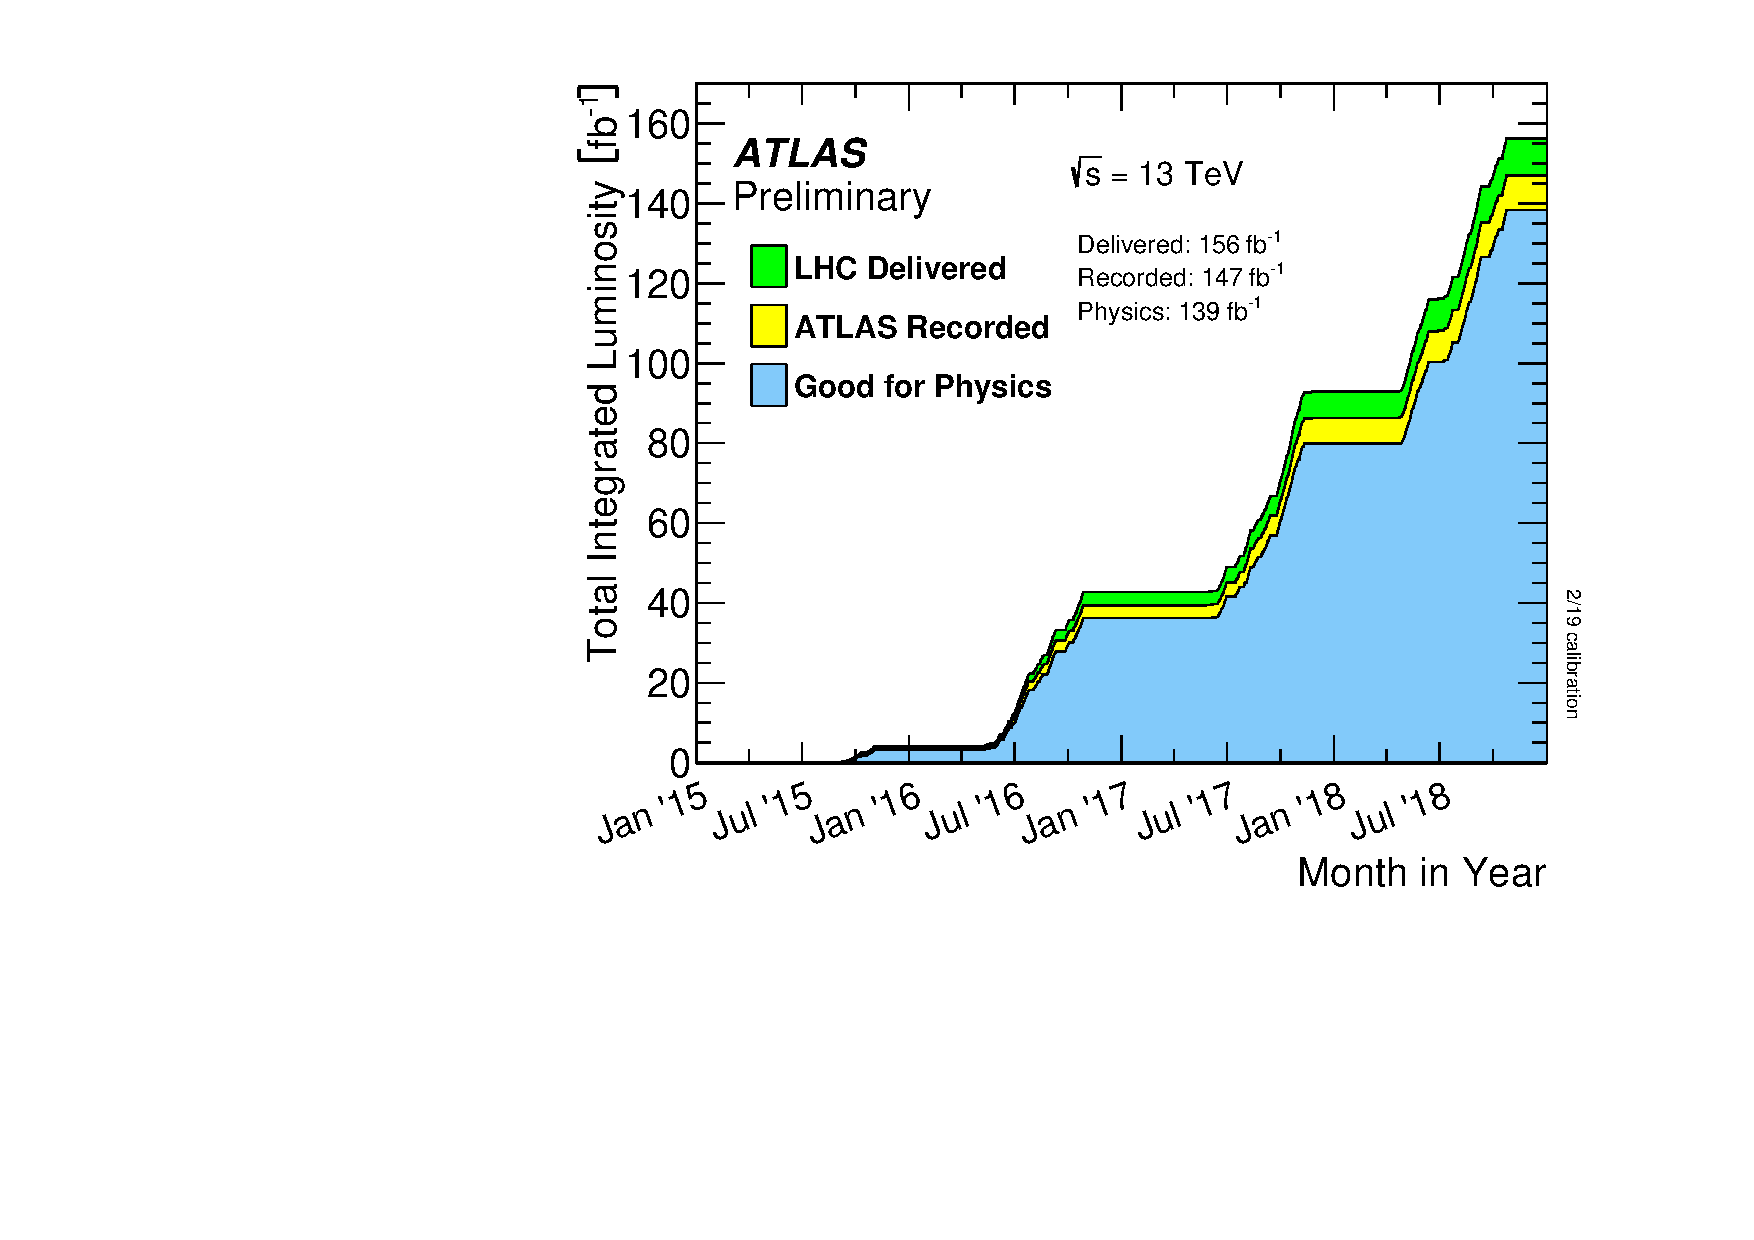
\includegraphics[width=0.8\textwidth]{figures/experiment/lhc/run2Lumi.pdf}
\caption{ (from: https://twiki.cern.ch/twiki/bin/view/AtlasPublic/LuminosityPublicResults)}
\label{fig:run2Lumi}
\end{figure}

The performance of the LHC during Run 2 enabled the machine to deliver a total of 156~\fb of collision data.
The total delivered integrated luminosity and that recorded by ATLAS are shown in Figure \ref{fig:run2Lumi}.
The number of commissioning days at the start of each year dropped from 58 down to 17, as the LHC was better understood.
Local optical corrections could be reused from year to year.
The maximum of bunches increased from 2244 up to 2556 per beam, and the stable beam efficiency increased from 35\% to 49\%.
During the run, UFO events occurred at rates of 1-20 per hour.
These and other run parameters are summarized in Table \ref{tab:run2}.

